% Options for packages loaded elsewhere
\PassOptionsToPackage{unicode}{hyperref}
\PassOptionsToPackage{hyphens}{url}
%
\documentclass[
]{article}
\usepackage{amsmath,amssymb}
\usepackage{iftex}
\ifPDFTeX
  \usepackage[T1]{fontenc}
  \usepackage[utf8]{inputenc}
  \usepackage{textcomp} % provide euro and other symbols
\else % if luatex or xetex
  \usepackage{unicode-math} % this also loads fontspec
  \defaultfontfeatures{Scale=MatchLowercase}
  \defaultfontfeatures[\rmfamily]{Ligatures=TeX,Scale=1}
\fi
\usepackage{lmodern}
\ifPDFTeX\else
  % xetex/luatex font selection
\fi
% Use upquote if available, for straight quotes in verbatim environments
\IfFileExists{upquote.sty}{\usepackage{upquote}}{}
\IfFileExists{microtype.sty}{% use microtype if available
  \usepackage[]{microtype}
  \UseMicrotypeSet[protrusion]{basicmath} % disable protrusion for tt fonts
}{}
\makeatletter
\@ifundefined{KOMAClassName}{% if non-KOMA class
  \IfFileExists{parskip.sty}{%
    \usepackage{parskip}
  }{% else
    \setlength{\parindent}{0pt}
    \setlength{\parskip}{6pt plus 2pt minus 1pt}}
}{% if KOMA class
  \KOMAoptions{parskip=half}}
\makeatother
\usepackage{xcolor}
\usepackage[margin=1in]{geometry}
\usepackage{color}
\usepackage{fancyvrb}
\newcommand{\VerbBar}{|}
\newcommand{\VERB}{\Verb[commandchars=\\\{\}]}
\DefineVerbatimEnvironment{Highlighting}{Verbatim}{commandchars=\\\{\}}
% Add ',fontsize=\small' for more characters per line
\usepackage{framed}
\definecolor{shadecolor}{RGB}{248,248,248}
\newenvironment{Shaded}{\begin{snugshade}}{\end{snugshade}}
\newcommand{\AlertTok}[1]{\textcolor[rgb]{0.94,0.16,0.16}{#1}}
\newcommand{\AnnotationTok}[1]{\textcolor[rgb]{0.56,0.35,0.01}{\textbf{\textit{#1}}}}
\newcommand{\AttributeTok}[1]{\textcolor[rgb]{0.13,0.29,0.53}{#1}}
\newcommand{\BaseNTok}[1]{\textcolor[rgb]{0.00,0.00,0.81}{#1}}
\newcommand{\BuiltInTok}[1]{#1}
\newcommand{\CharTok}[1]{\textcolor[rgb]{0.31,0.60,0.02}{#1}}
\newcommand{\CommentTok}[1]{\textcolor[rgb]{0.56,0.35,0.01}{\textit{#1}}}
\newcommand{\CommentVarTok}[1]{\textcolor[rgb]{0.56,0.35,0.01}{\textbf{\textit{#1}}}}
\newcommand{\ConstantTok}[1]{\textcolor[rgb]{0.56,0.35,0.01}{#1}}
\newcommand{\ControlFlowTok}[1]{\textcolor[rgb]{0.13,0.29,0.53}{\textbf{#1}}}
\newcommand{\DataTypeTok}[1]{\textcolor[rgb]{0.13,0.29,0.53}{#1}}
\newcommand{\DecValTok}[1]{\textcolor[rgb]{0.00,0.00,0.81}{#1}}
\newcommand{\DocumentationTok}[1]{\textcolor[rgb]{0.56,0.35,0.01}{\textbf{\textit{#1}}}}
\newcommand{\ErrorTok}[1]{\textcolor[rgb]{0.64,0.00,0.00}{\textbf{#1}}}
\newcommand{\ExtensionTok}[1]{#1}
\newcommand{\FloatTok}[1]{\textcolor[rgb]{0.00,0.00,0.81}{#1}}
\newcommand{\FunctionTok}[1]{\textcolor[rgb]{0.13,0.29,0.53}{\textbf{#1}}}
\newcommand{\ImportTok}[1]{#1}
\newcommand{\InformationTok}[1]{\textcolor[rgb]{0.56,0.35,0.01}{\textbf{\textit{#1}}}}
\newcommand{\KeywordTok}[1]{\textcolor[rgb]{0.13,0.29,0.53}{\textbf{#1}}}
\newcommand{\NormalTok}[1]{#1}
\newcommand{\OperatorTok}[1]{\textcolor[rgb]{0.81,0.36,0.00}{\textbf{#1}}}
\newcommand{\OtherTok}[1]{\textcolor[rgb]{0.56,0.35,0.01}{#1}}
\newcommand{\PreprocessorTok}[1]{\textcolor[rgb]{0.56,0.35,0.01}{\textit{#1}}}
\newcommand{\RegionMarkerTok}[1]{#1}
\newcommand{\SpecialCharTok}[1]{\textcolor[rgb]{0.81,0.36,0.00}{\textbf{#1}}}
\newcommand{\SpecialStringTok}[1]{\textcolor[rgb]{0.31,0.60,0.02}{#1}}
\newcommand{\StringTok}[1]{\textcolor[rgb]{0.31,0.60,0.02}{#1}}
\newcommand{\VariableTok}[1]{\textcolor[rgb]{0.00,0.00,0.00}{#1}}
\newcommand{\VerbatimStringTok}[1]{\textcolor[rgb]{0.31,0.60,0.02}{#1}}
\newcommand{\WarningTok}[1]{\textcolor[rgb]{0.56,0.35,0.01}{\textbf{\textit{#1}}}}
\usepackage{graphicx}
\makeatletter
\def\maxwidth{\ifdim\Gin@nat@width>\linewidth\linewidth\else\Gin@nat@width\fi}
\def\maxheight{\ifdim\Gin@nat@height>\textheight\textheight\else\Gin@nat@height\fi}
\makeatother
% Scale images if necessary, so that they will not overflow the page
% margins by default, and it is still possible to overwrite the defaults
% using explicit options in \includegraphics[width, height, ...]{}
\setkeys{Gin}{width=\maxwidth,height=\maxheight,keepaspectratio}
% Set default figure placement to htbp
\makeatletter
\def\fps@figure{htbp}
\makeatother
\setlength{\emergencystretch}{3em} % prevent overfull lines
\providecommand{\tightlist}{%
  \setlength{\itemsep}{0pt}\setlength{\parskip}{0pt}}
\setcounter{secnumdepth}{-\maxdimen} % remove section numbering
\newlength{\cslhangindent}
\setlength{\cslhangindent}{1.5em}
\newlength{\csllabelwidth}
\setlength{\csllabelwidth}{3em}
\newlength{\cslentryspacingunit} % times entry-spacing
\setlength{\cslentryspacingunit}{\parskip}
\newenvironment{CSLReferences}[2] % #1 hanging-ident, #2 entry spacing
 {% don't indent paragraphs
  \setlength{\parindent}{0pt}
  % turn on hanging indent if param 1 is 1
  \ifodd #1
  \let\oldpar\par
  \def\par{\hangindent=\cslhangindent\oldpar}
  \fi
  % set entry spacing
  \setlength{\parskip}{#2\cslentryspacingunit}
 }%
 {}
\usepackage{calc}
\newcommand{\CSLBlock}[1]{#1\hfill\break}
\newcommand{\CSLLeftMargin}[1]{\parbox[t]{\csllabelwidth}{#1}}
\newcommand{\CSLRightInline}[1]{\parbox[t]{\linewidth - \csllabelwidth}{#1}\break}
\newcommand{\CSLIndent}[1]{\hspace{\cslhangindent}#1}
\usepackage{booktabs}
\usepackage{longtable}
\usepackage{array}
\usepackage{multirow}
\usepackage{wrapfig}
\usepackage{float}
\usepackage{colortbl}
\usepackage{pdflscape}
\usepackage{tabu}
\usepackage{threeparttable}
\usepackage{threeparttablex}
\usepackage[normalem]{ulem}
\usepackage{makecell}
\usepackage{xcolor}
\ifLuaTeX
  \usepackage{selnolig}  % disable illegal ligatures
\fi
\IfFileExists{bookmark.sty}{\usepackage{bookmark}}{\usepackage{hyperref}}
\IfFileExists{xurl.sty}{\usepackage{xurl}}{} % add URL line breaks if available
\urlstyle{same}
\hypersetup{
  pdftitle={My first notebook},
  pdfauthor={Chandan Kumar Pandey},
  hidelinks,
  pdfcreator={LaTeX via pandoc}}

\title{My first notebook}
\author{Chandan Kumar Pandey}
\date{2023-10-12}

\begin{document}
\maketitle

\hypertarget{activity-uno}{%
\section{Activity uno}\label{activity-uno}}

\hypertarget{advantage-of-r-markdown}{%
\subsection{Advantage of R Markdown}\label{advantage-of-r-markdown}}

\hypertarget{question-1--does-the-number-of-hours-students-study-impact-their-grades}{%
\subsubsection{Question 1:- Does the number of hours students study
impact their
grades?}\label{question-1--does-the-number-of-hours-students-study-impact-their-grades}}

\hypertarget{introduction}{%
\paragraph{Introduction}\label{introduction}}

You can write your introduction here

\hypertarget{method-hypothetical}{%
\paragraph{Method (Hypothetical)}\label{method-hypothetical}}

We conducted a survey in schools of Bangalore North Taluk to understand
the impact of the number of hours of study on student final scores.
Student's parents were interviewed during parent-teacher meetings (PTA)
to collect data on number of hours the child. Further from the school
records, we collected overall final grades. To assess the impact of
study time and course taken on the overall grades, we fitted a linear
regression model with the number of hours as the independent variable
and number of courses enrolled in and marks are response
variable;(\(marks=\beta_1*Number of course +\beta_2 * Hours study + \epsilon\)),
where \(\epsilon~N(0,1)\) . All analyses were performed in R statistical
software R version 4.1.2 (2021-11-01) (R Core Team (2019)).

\hypertarget{results}{%
\paragraph{Results}\label{results}}

A total of 100 student records were collected, with the number of
courses students were enrolled in ranging between 3 and 8. Based on
parents' interviews, on average, students studied for 4.08 hours per day
(ranging from 0.1 to 7.96 per day). Further, the average mark scored was
24.42 in log scale, ranging from 5.61 to 55.3..

\begin{Shaded}
\begin{Highlighting}[]
\NormalTok{model }\OtherTok{\textless{}{-}} \FunctionTok{lm}\NormalTok{(Marks}\SpecialCharTok{\textasciitilde{}}\NormalTok{number\_courses}\SpecialCharTok{+}\NormalTok{time\_study,}\AttributeTok{data =}\NormalTok{ student\_marks)}
\NormalTok{anova\_table }\OtherTok{\textless{}{-}} \FunctionTok{anova}\NormalTok{(model)}\SpecialCharTok{\%\textgreater{}\%}\FunctionTok{as.data.frame}\NormalTok{()}\SpecialCharTok{\%\textgreater{}\%}\FunctionTok{round}\NormalTok{(}\DecValTok{3}\NormalTok{)}
\NormalTok{model\_summary }\OtherTok{\textless{}{-}} \FunctionTok{summary}\NormalTok{(model)}
\NormalTok{summary\_table }\OtherTok{\textless{}{-}}\NormalTok{ model\_summary}\SpecialCharTok{$}\NormalTok{coefficients}\SpecialCharTok{\%\textgreater{}\%}\FunctionTok{as.data.frame}\NormalTok{()}\SpecialCharTok{\%\textgreater{}\%}\FunctionTok{round}\NormalTok{(}\DecValTok{3}\NormalTok{)}
\FunctionTok{rownames}\NormalTok{(summary\_table) }\OtherTok{\textless{}{-}} \FunctionTok{c}\NormalTok{(}\StringTok{"Intercept"}\NormalTok{,}\StringTok{"Courses enrolled{-}in"}\NormalTok{,}\StringTok{"Per day hours of study"}\NormalTok{)}
\end{Highlighting}
\end{Shaded}

In our model, the number of
courses(1,283.298,\textbf{\emph{p\textless0.005}} ) and study times
(1,1246.281,\textbf{\emph{p\textless0.005}} )were significant in
explaining the student's grades in the final examination (\textbf{Table
1}). Overall, our model was able to explain 93.91\% of the variation in
the marks of students. With the increase in each course, the student
average grades improved by -7.456(1.174). Similarly, each extra hour of
study will increase the score by a factor of 1.864(0.202) (Table 2,
Fig1)

\begin{verbatim}
## 
## Attaching package: 'kableExtra'
\end{verbatim}

\begin{verbatim}
## The following object is masked from 'package:dplyr':
## 
##     group_rows
\end{verbatim}

\begin{table}

\caption{\label{tab:tables1 in latex}Table1: Annova output of the model}
\centering
\resizebox{\linewidth}{!}{
\begin{tabular}[t]{lrrrrr}
\toprule
  & Df & Sum Sq & Mean Sq & F value & Pr(>F)\\
\midrule
\cellcolor{gray!6}{number\_courses} & \cellcolor{gray!6}{1} & \cellcolor{gray!6}{3538.880} & \cellcolor{gray!6}{3538.880} & \cellcolor{gray!6}{283.298} & \cellcolor{gray!6}{0}\\
time\_study & 1 & 15568.180 & 15568.180 & 1246.281 & 0\\
\cellcolor{gray!6}{Residuals} & \cellcolor{gray!6}{97} & \cellcolor{gray!6}{1211.696} & \cellcolor{gray!6}{12.492} & \cellcolor{gray!6}{NA} & \cellcolor{gray!6}{NA}\\
\bottomrule
\end{tabular}}
\end{table}

\begin{table}

\caption{\label{tab:addition table 2 latex}Table2: model summary}
\centering
\resizebox{\linewidth}{!}{
\begin{tabular}[t]{lrrrr}
\toprule
  & Estimate & Std. Error & t value & Pr(>|t|)\\
\midrule
\cellcolor{gray!6}{Intercept} & \cellcolor{gray!6}{-7.456} & \cellcolor{gray!6}{1.174} & \cellcolor{gray!6}{-6.349} & \cellcolor{gray!6}{0}\\
Courses enrolled-in & 1.864 & 0.202 & 9.243 & 0\\
\cellcolor{gray!6}{Per day hours of study} & \cellcolor{gray!6}{5.399} & \cellcolor{gray!6}{0.153} & \cellcolor{gray!6}{35.303} & \cellcolor{gray!6}{0}\\
\bottomrule
\end{tabular}}
\end{table}

\begin{figure}
\centering
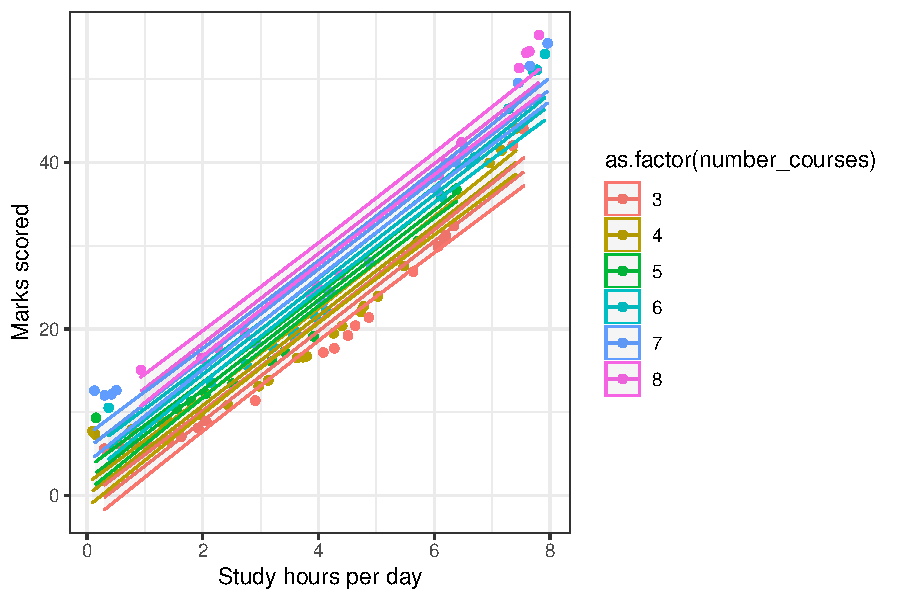
\includegraphics{Workshop_mark_down_files/figure-latex/graphs-1.pdf}
\caption{Student performace in relation to number of hours study and
courses enrolled in}
\end{figure}

\hypertarget{discussion}{%
\paragraph{Discussion}\label{discussion}}

\begin{enumerate}
\def\labelenumi{\arabic{enumi}.}
\tightlist
\item
  Our study align with results of Yu (2011) and Borg \emph{et al.}
  (1989) that with more study we can get good grades
\item
  It was surprising that several courses also increased the overall
  mark. This may be due to the following reasons

  \begin{itemize}
  \tightlist
  \item
    Generally, people who study more take more courses.
  \item
    The average of many subjects compensates for few bad results.
  \end{itemize}
\end{enumerate}

References:

\hypertarget{refs}{}
\begin{CSLReferences}{0}{0}
\leavevmode\vadjust pre{\hypertarget{ref-borg1989case}{}}%
\textsc{Borg M.O.}, \textsc{Mason P.M.} \& \textsc{Shapiro S.L.} 1989.
--- The case of effort variables in student performance. \emph{The
Journal of Economic Education} 20 (3): 308--313

\leavevmode\vadjust pre{\hypertarget{ref-R-base}{}}%
\textsc{R Core Team} 2019. --- \emph{\href{https://www.R-project.org}{R:
A language and environment for statistical computing}}. Vienna, Austria,
R Foundation for Statistical Computing.

\leavevmode\vadjust pre{\hypertarget{ref-yu2011much}{}}%
\textsc{Yu D.D.} 2011. --- How much do study habits, skills, and
attitudes affect student performance in introductory college accounting
courses?

\end{CSLReferences}

\end{document}
